%------------------Ejercicio 1--------------------------------

\begin{question}
    Sean  $V=\{ (x,y,z) \in \mathbb{R}^{3}:  x\leq 0, \;  y
        \leq 0, \;  0 \leq  z \leq 1-x^{2}-y^{2}  \}$ y
    $S=\{ (x,y,z) \in \mathbb{R}^{3}:  x\geq 0, \; y \geq 0,
        z\geq 0,\;  z = 1-x^{2}-y^{2}  \}$.
    Calcluar el volumen de $V$ y el \'area de $S$.
\end{question}

%------------------Ejercicio 2--------------------------------

\begin{question}
    Sean  $S$ una superficie  esf\'erica de radio $R$ con
    centro en el primer octante  y  $\mathbf{F}$ un campo de
    clase $C^{1}$  con $\nabla\cdot\mathbf{F}(x,y,z) = x+y+z$.
    Probar que  el flujo saliente de $\mathbf{F}$ a trav\'es de
    $S$  es no negativo.
\end{question}

%------------------Ejercicio 3--------------------------------

\begin{question}
    Sean  $C$ el borde del tri\'angulo de v\'ertices $(-1,0)$,
    $(1,0)$ y $(0,1)$ y el campo $\mathbf{F}(x,y) =
        \Big(e^{\cos(x)+x^{2}}+xy^{2}+2y, \ln(1+e^{y^{2}}) +yx^{2}+3x \Big).$
    Calcular,  indicando la orientaci\'on elegida:
    $$ \int_{C} \mathbf{F}\cdot ds$$
\end{question}

%------------------Ejercicio 4--------------------------------

\begin{question}
    Probar que el campo $\mathbf{F}(x,y) = \Big(y e^{xy}+y\cos(xy)
        ,xe^{xy}+\cos(xy) x \Big)$ es conservativo.  Dada $C$ la curva
    parametrizada por $\boldsymbol{\alpha}(t) = (t^{2},t)$ con $t
        \in [0,1]$ calcular el trabajo realizado por $\mathbf{F}$ sobre $C.$
\end{question}

\newpage

%------------------Solucion 1--------------------------------

\begin{solution}
    Nos piden calcular $\iiint_V dV$ y $\iint_S dA$. Para la
    integral de volumen conviene trabajar en coordenadas
    cil\'indricas y para la de superficie habr\'a que parametrizar.

    \begin{center}
        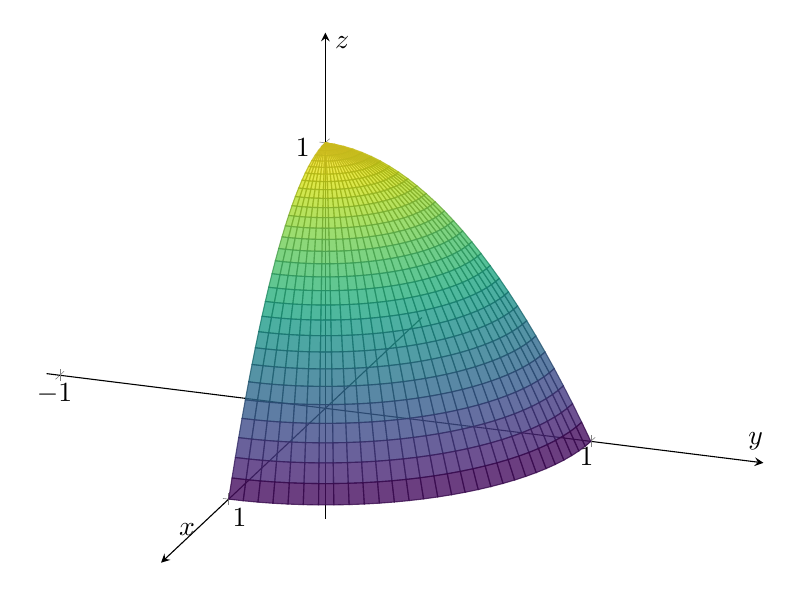
\begin{tikzpicture}
          \begin{axis}[
                axis lines=center,
                axis equal,
                view={110}{20},
                xlabel=$x$,
                ylabel=$y$,
                zlabel=$z$,
                xtick={1},
                ytick={-1,1},
                ztick={1,1.5},
                xmin=-1,
                ymin=-0.5,
                zmin=0,
                xmax=1.7,
                ymax=1.1,
                zmax=1,
                samples=30,
                width=14cm,
                height=12cm,
                colormap/viridis,
                xlabel style={at={(0.31,0.2)}},
            ]
            \addplot3 [surf, opacity=0.8, draw=none, restrict z to domain=0:1,
            data cs=polar, domain=0:90, y domain=0:1] (x, y, 1-y^2);
          \end{axis}
        \end{tikzpicture}
      \end{center}

    Aplicando la transformaci\'on $V \rightarrow V^*$ queda
    \begin{align*}
        V^*      & =\{(\rho, \phi, z)\in\Re^3: \rho\cos\phi \leq 0,\;
        \rho\sen\phi \leq 0,\; 0 \leq z \leq 1-\rho^2\}               \\
        \iff V^* & =\{(\rho, \phi, z)\in\Re^3: \pi \leq \phi \leq
        \frac{3}{2}\pi,\; 0 \leq z \leq 1,\; 0 \leq \rho \leq
        \sqrt{1-z} \}.
    \end{align*}
    Y por el teorema de cambio de variable tenemos que
    \begin{align*}
        \iiint_V dV & = \iiint_{V^*} \rho\:dV = \int_\pi^{\frac{3}{2}\pi}
        \int_0^1\int_0^{\sqrt{1-z}}\rho\:d\rho dz d\phi                   \\
                    & =\frac{\pi}{2}\int_0^1\frac{1}{2}(1-z)\:dz =
        \frac{\pi}{8}.
    \end{align*}

    Para parametrizar $S$, llamamos
    \[
        D = \{(\rho, \phi)\in\Re^2 : \pi\leq\phi\leq\frac{3}{2}\pi,\;
        0\leq\rho\leq 1\}.
    \]
    y
    \[
        \boldsymbol{\Sigma}:D\subset\Re^2\rightarrow\Re^3\text{ tal que }
        \boldsymbol{\Sigma}(\rho,\phi)=(\rho\cos\phi,\;\rho\sen\phi,\;\rho^2).
    \]
    Calculamos las derivadas paraciales de $\boldsymbol{\Sigma}$.
    \begin{align*}
        \boldsymbol{\Sigma}_{\rho}&=(\cos \phi,\;\sen \phi,\; 2\rho)\\
        \boldsymbol{\Sigma}_\phi&=(  -\rho \sen \phi,\;\rho \cos \phi,\;0)
        \end{align*}
    Luego
    $$
        \boldsymbol{\Sigma}_{\rho} \times\boldsymbol{\Sigma}_\phi =
        (-2\rho^2 \cos\phi  , \;-2\rho^2 \sen \phi, \;\rho),
    $$ 
    $$\|\boldsymbol{\Sigma}_{\rho} \times\boldsymbol{\Sigma}_\phi\|
        = \rho\sqrt{4\rho^2+1}.
    $$ 
    Entonces escribimos, por definici\'on, el \'area de $S$ como
    \[
        \iint_S dA = \iint_D \| \boldsymbol{\Sigma}_{\rho}
        \times\boldsymbol{\Sigma}_\phi\|\:d\rho d\phi = \int_\pi^{\frac{3}{2}\pi}\int_0^1\rho\sqrt{4\rho^2+1}\:d\rho d\phi.
    \]
    Nos queda la misma integral que \eqref{eq:integral1}, s\'olo que con distintos l\'imites de integraci\'on. Por lo que, procediendo de la misma manera, sustituyendo $u = 4\rho^2+1$, obtenemos
    \begin{gather*}
        \iint_S dA =
        \frac{1}{8}\int_\pi^{\frac{3}{2}\pi}\int_1^5\sqrt{u}\:du =
        \frac{\pi}{16}\frac{u^{\frac{3}{2}}}{\frac{3}{2}}\Bigg\lvert_1^5 =
        \frac{\pi}{24}(\sqrt{125}-1).
    \end{gather*}
\end{solution}

%------------------Solucion 2--------------------------------

\begin{solution}
    Tenemos que $S=\{(x,y,z)\in\Re^3:
        (x-x_0)^2+(y-y_0)^2+(z-z_0)^2=R^2\}$, con $R>0$ y
    $(x_0,y_0,z_0)$ en el primer octante.
    Por el teorema de la divergencia
    \begin{equation}
        \iint_S \mathbf{F}\cdot\:d\mathbf{A} = \iiint_\Omega
        \nabla\cdot\mathbf{F}\:dV
        = \iiint_\Omega (x+y+z)\:dxdydz, \label{eq: divEj2}
    \end{equation}
    tomando la orientaci\'on de $S$ como exterior.

    Aplicando una tranformaci\'on a coordenadas esf\'ericas, tal que
    \begin{align*}
        x & =\rho\sen\phi\cos\theta+x_0 \\
        y & =\rho\sen\phi\sen\theta+y_0 \\
        z & =\rho\cos\phi+z_0,
    \end{align*}
    nos queda el conjunto $S^*$
    \[
        S^*=\{(\rho,\phi,\theta)\in\Re^3:0\leq\rho\leq R,\;
        0\leq\theta\leq2\pi,\;0\leq\phi\leq\pi\}.
    \]
    De la ecuaci\'on \eqref{eq: divEj2} y usando el teorema
    de cambio de variable,
    \begin{gather*}
        \iiint_\Omega (x+y+z) \:dV = \iiint_{\Omega^*}
        (\rho\sen\phi\cos\theta + \rho\sen\phi\sen\theta
        + \rho\cos\phi + x_0 + y_0 + z_0)
        \:\rho^2\sen\phi\:d\rho d\theta d\phi=\\
        = \int_0^\pi\int_0^{2\pi}\int_0^R (\rho\sen\phi\cos\theta
        + \rho\sen\phi\sen\theta + \rho\cos\phi
        + x_0 + y_0 + z_0)\rho^2\sen\phi\:d\rho d\theta d\phi.
    \end{gather*}
    Al distribuir el $\rho^2\sen\phi$ entre los primeros dos
    t\'erminos, queda para estos \(\rho^3\sen\phi^2\cos\theta\) y \\
    \(\rho^3\sen\phi^2\sen\theta\); que al integrarlos entre 0
    y $2\pi$, con respecto a $\theta$, se anulan. Entonces queda,
    distribuyendo la suma del integrando,
    \[
        \int_0^\pi\int_0^{2\pi}\int_0^R \rho^3\cos\phi\sen\phi\:
        d\rho d\theta d\phi + \int_0^\pi\int_0^{2\pi}\int_0^R
        (x_0 + y_0 + z_0)\rho^2\sen\phi\:d\rho d\theta d\phi.
    \]
    A su vez, la primer integral es 0 porque al integrar una
    funci\'on peri\'odica impar, $\cos\phi\sen\phi$, en un
    semi per\'iodo \'esta se anula. Por \'ultimo queda
    \[
        (x_0 + y_0 + z_0)\int_0^\pi\int_0^{2\pi}\int_0^R
        \rho^2\sen\phi\:d\rho d\theta d\phi = (x_0 + y_0 + z_0)
        \frac{4}{3}\pi R^3 > 0,
    \]
    pues $(x_0, y_0, z_0)$ pertenece al primer octante.
    Por lo que queda demostrado que el flujo es positivo.

    \textcolor{red}{por qu\'e ser\'ia -no negativo-? por ej. 
    cuando R = 0 o cuando el centro de la esfera es el origen es = 0}
\end{solution}

%------------------Solucion 3--------------------------------

\begin{solution}
    Nos piden integrar sobre la siguiente curva $C$.

    \begin{center}
        \begin{tikzpicture}
            \begin{axis}[
                    axis lines=center,
                    axis equal,
                    xlabel=$x$, ylabel=$y$,
                    xmin=-1.5, xmax=1.5,
                    ymin=0, ymax=1,
                    xtick distance=1, ytick distance=1,
                ]
                \draw[cyan, thick] (-1,0) -- (1,0) -- (0,1) -- cycle;
            \end{axis}
        \end{tikzpicture}
    \end{center}

    Tomamos la orientaci\'on de $C$ como antihoraria.
    % depende de como este definido el interior de una curva
    Dado que el tri\'angulo $T$  es simplemente conexo,   $T
        \in \text{dom}(\mathbf{F})$ y $\mathbf{F}\in C^1$, entonces
    por el teorema de Green
    \[
        \oint_C \mathbf{F}\cdot d\mathbf{s} = \iint_T
        \nabla\times\mathbf{F}\:dA.
    \]
    Como $\nabla\times\mathbf{F} = 1$, queda que \[\oint_C
        \mathbf{F}\cdot d\mathbf{s} = \iint_T dA = \textcolor{red}{Area}(T)
        = \frac{2\cdot1}{2} = 1.\]
\end{solution}

%------------------Solucion 4--------------------------------

\begin{solution}
    Ya que nos piden demostrar que $\mathbf{F}$ es conservativo
    y calcular una integral de l\'inea sobre una curva no
    cerrada nos conviene buscar, si es que existe, la funci\'on
    potencial de $\mathbf{F}$. Nos encontramos con la ecuaci\'on
    $\nabla f = \mathbf{F}$, la cual describe el siguiente
    sistema de ecuaciones diferenciales.
    \[
        \begin{dcases}
            f_x(x,y) = ye^{xy} + y \cos{(xy)} \\[.2cm]
            f_y(x,y) = xe^{xy} + x \cos{(xy)}
        \end{dcases}
    \]
    Mirando cada t\'ermino detenidamente se puede llegar a
    la conclusi\'on de que $$f(x,y) = e^{xy} + \sen{(xy)} + C,
        \mbox{ con } C\in\Re$$ es soluci\'on del sistema. Lo que
    significa que $\mathbf{F}$ es un campo conservativo.

    Luego para calcular $\int_C \mathbf{F}\cdot d\mathbf{s}$
    utilizamos el siguiente teorema.
    \[
        \int_C \nabla f\cdot d\mathbf{s} =
        f(\boldsymbol{\alpha}(1)) - f(\boldsymbol{\alpha}(0)) =
        f((1,1)) - f((0,0)) = e + \sen1 - 1.
    \]
\end{solution}


